%% LyX 2.1.4 created this file. For more info, see http://www.lyx.org/.
%% Do not edit unless you really know what you are doing.
\documentclass{article}
\usepackage[latin9]{inputenc}
\usepackage{amsmath}
\usepackage{graphicx}
%\usepackage{float} if use H in floats with this included, floats go exactly where placed
\begin{document}

\title{\textbf{Programming 2 Assignment}}


\author{Gerald Hu, Aaron Skouby \\
\\
CSCE 221-200}


\date{March 11, 2016}

\maketitle

\section*{Introduction}

The purpose of this assignment was to increase the understanding of data structures and implementations that were discussed in class. Specifically, the project explored implementing a map ADT using a binary tree. The performance of the operations of the map were analyzed for both a binary search tree implementation and an AVL binary tree implementation. Functionality was written for the map that allowed it to insert, delete, access, and edit key-value pairs. Additionally, some lower level details on the tree representation itself were implemented. This includes functions that allowed searching, inserting, and deleting from the underlying tree as well as rebalancing the tree after these insertions and deletions. The results of this lab basically demonstrated the theoretical performance analysis that was determined in class for the binary search tree and the AVL tree. The running time of the insertions, searches, and deletions are all the same as each other because they are based of the height of the tree. The best case and average case for both types of tree was $O(\log{n})$. The difference existed in the worst case scenario. For the AVL tree this was still $O(\log{n})$, but for binary search trees is was $O(n)$. The AVL tree did its job of making sure that the worst case is still $O(\log{n})$

\section*{Implementation Details}

The map was implemented with a binary search tree, using the AVL method of self-balancing. The tree had node data members, a size\_t ``sz'' which kept track of the size of the tree, special ``leaf'' nodes at the end of each branch with no key or value, and a special ``superroot'' node whose left subtree was the main tree and a null parent. Each node of the tree stored pointers to its parent, left child, and right child, as well as storing a pair called ``value''. This pair was the main data element of the node, storing the key, or index, in its first position, and the data value in its second position. The pair used the standard template library pair. \\


\noindent The map had two erase functions, one which took a key, one which took an iterator for position. These would take a key or iterator and find the desired node, and would get a pointer to it. Then, it would pass the node pointer to a helper function eraser(node{*} n), which would find the node (or otherwise do nothing), remove it, place the child in the proper position, and return the next node in an in-order traversal. Insert functions were implemented similar to the eraser functions. There were two insert functions with one taking a key, one taking an iterator, and both being based on an inserter helper function. The inserter function would take a key and value, and would either construct a new node and add it to the map; or, in the case where the key already existed in a map, replace that key's value with the new value.\\


\noindent The map's size was automatically adjusted by the helper functions eraser() and inserter() when needed. Both eraser() and inserter() called rebalance() to fix tree imbalances after doing their respective operation. Rebalance() would scan up the tree to find imbalances, and call the restructure() function on them, making appropriate left or right rotations to maintain the balance conditions of having the maximum difference between the left and right subtrees of any node be 1.\\


\noindent Timing.cpp was essentially unchanged from the code provided
by the instructors. The timing function was already implemented, and
for the most part our tests simply changed the parameters of the function.
This timing function relies on high\_resolution\_clock; given a map
and a number, the function would repeatedly push random elements into
the map the specified number of times.\\



\section*{Theoretical Analysis}

\noindent For insert and erase operations on a simple binary search tree, the worst case occurs when the position to insert the node or of the node to be erased is at the bottom of the tree. This means that function must traverse the entire tree's height before it can perform its operation. The tree's height can change, varying from $O(\log{n})$ to $O(n)$, but the performance of the insert and erase functions will always depend on the height. Thus, the insert and erase functions are $O(h)$, where $h$ is the height of the tree.\\

\noindent The rebalancing on an AVL tree is based of the linked-node implementation. A single restructure around one node is O(1) because it is simply reassigning the pointers of three nodes. Rebalance() travels up the entire tree's height to ensure that all nodes above the changed point are balanced, which is $O(h)$. The cumulative restructure is O(1){*}O(h)) = O(h). For AVL trees, for which restructure exists, the height will be $O(\log{n})$, so the rebalance is $O(\log{n})$.\\

\noindent For the insert and erase operations on an AVL tree there is a logarithmic bound on the height of the tree. Since the insert and delete functions are the same as for a regular binary search tree except that they rebalance, which is $O(h)$ , their performance is still $O(h)$ because $O(h+h)$ is $O(h)$. The logarithmic bound thus arises from a logarithmic bound on the height of an AVL tree. To prove this, begin with a function $n(h)$ that returns the minimum number of internal nodes of an AVL tree with height $h$. Note that an AVL tree wiith the minimum number of nodes for that height contains a root node, the minimal subtree of height $h-1$, and the minimal subtree of height $h-2$. That means that $n(h)$ for the tree is $1+n(h-1)+n(h-2)$. Because it a node has to be added to get from the minimal tree with height $h-2$ to the minimal tree with height $h-1$, $n(h-1) > n(h-2)$. Substituting that fact into the equation for $n(h)$, the expression $1+n(h-1)+n(h-2)>2n(h-2)$ is obtained. As a result, $n(h)>2n(h-2)$. By extending this fact back recursively, $2n(h-2)$ can be substituted with $4n(h-4)$, and and so on until the patern $n(h)>2^{i}n(h-2i)$ is determined. \\


\noindent When evaluating this for the base case of $n(1)=1$, an AVL tree with
height 1. Substituting that in and solving for $i$ gives $i=(\frac{h}{2}-1)$. This produces $n(h)>2^{\frac{h}{2}-1}$,
which can be rearranged to $h<2(log(n(h)))+2$, which is a logarithmic bound on the height of the AVL trees.\\



\section*{Experimental Setup}

Timing tests were conducted using the provided timing.cpp, compiled
with the provided makefile's commands. Compilation was done on the
``linux.cse.tamu.edu'' server, with G++ version 4.7.3 (SUSE Linux)
(found via g++ --version). Compilation was set to the C++11 standard,
with the -G flag enabled and O2 optimization level, warnings set to
-Wall -Werror (all warnings treated as compilation errors), and dependencies
flagged with -MMD (auto-generate dependencies).\\


\noindent Tests were run on the ``compute.cse.tamu.edu'' server,
which runs Arch Linux x86\_64 version 8.12 (found via arch --version
and lsb\_release -a). This server has 99026668 total kilobytes of
RAM (found via free). It uses Intel Core i7-3970X CPUs (2 sockets,
8 cores per socket, 2 threads per core), with a clock speed of 2000
mHz (found via lscpu). Each core has a Xeon E5-2650 processor (found
via lshw --short).\\


\noindent Timing functions output timing results for input sizes that were
powers of 2, starting from 2 itself, and ending at a maximum size
specified by the user. Each step of the timing was repeated 10 times,
and the average of each result taken. Linear height n inserts went
up to a maximum input size of 32768; logarithmic height n inserts
went up to a maximum input size of 4194304, and random n inserts went
up to a maximum input size of 1048576.\\


\noindent timing.o was run twice: first on a tree with AVL rebalancing and then on a simpler binary tree with no rebalancing method. These results for the performance were then compared between the two trees.


\section*{Results and Discussion}

In testing the timing performance of the functions for the binary search tree and AVL tree implementations of the map ADT, only the insert function was tested. As was discussed in the theoretical analysis section, all of the three main functions of the map ADT (find, insert, snd erase) for the binary search tree and AVL tree have the same asymptotic running time. As a result it is only necessary to test one of the functions because the results should be asymptotically the same for the other two as well. \\


\begin{figure}[h]
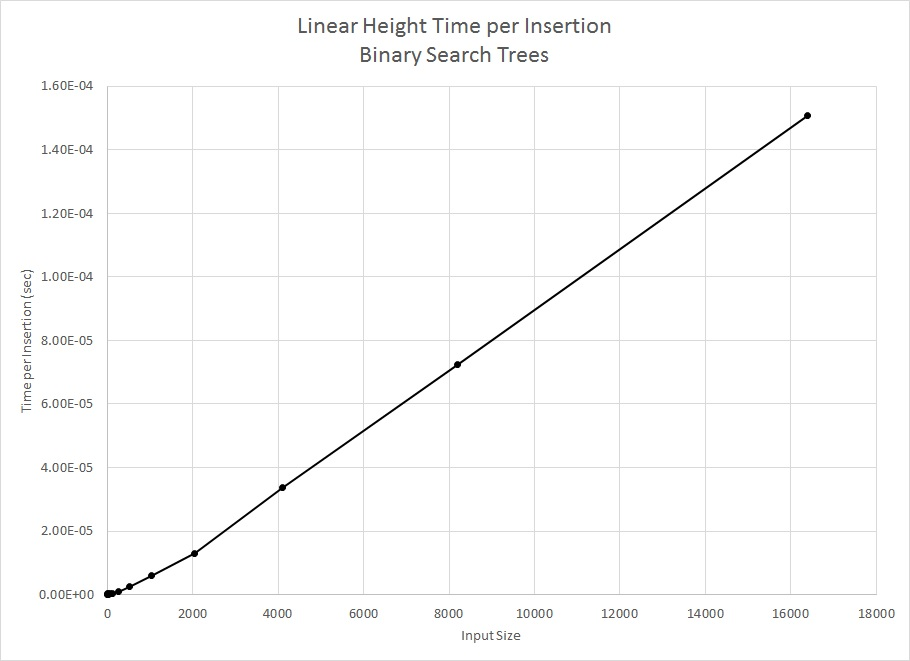
\includegraphics[width=11cm]{report/Linear_Time_Per_(Binary)} \caption{Graph of the Time Taken per Addition for Different Input Sizes for
a Linear Order Added Binary Search Tree}
\label{fig:Linear_Time_Per_Binary} 
\end{figure}


\begin{figure}[h]
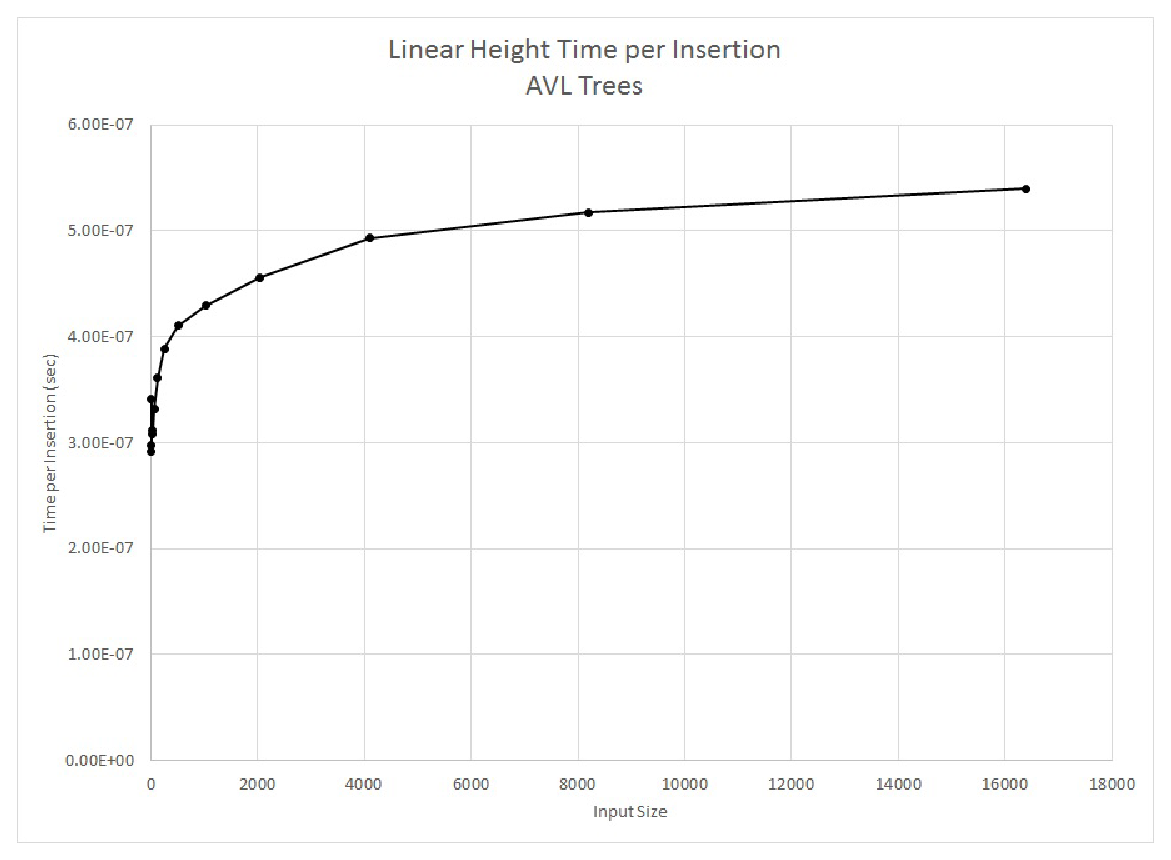
\includegraphics[width=11cm]{report/Linear_Time_Per_(AVL)} \caption{Graph of the Time Taken for Different Input Sizes for a Linear Order
Added AVL Tree}
\label{fig:Linear_Time_Per_AVL} 
\end{figure}


\begin{figure}[h]
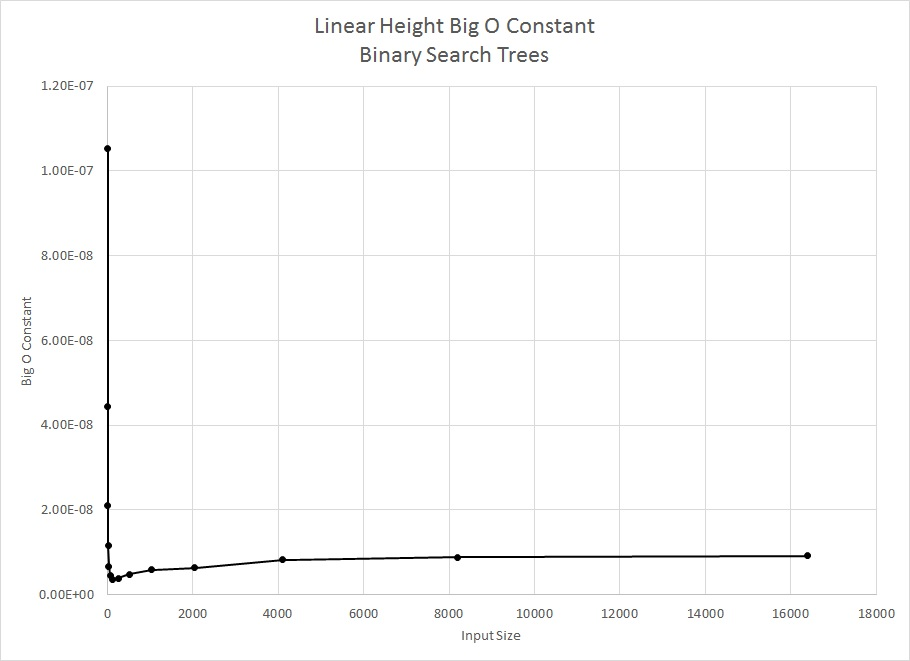
\includegraphics[width=11cm]{report/Linear_Big_O_(Binary)} \caption{Graph of the Big O Constants for Different Input Sizes for a Linear
Order Added Binary Search Tree}
\label{fig:Linear_Big_O_Binary} 
\end{figure}


\begin{figure}[h]
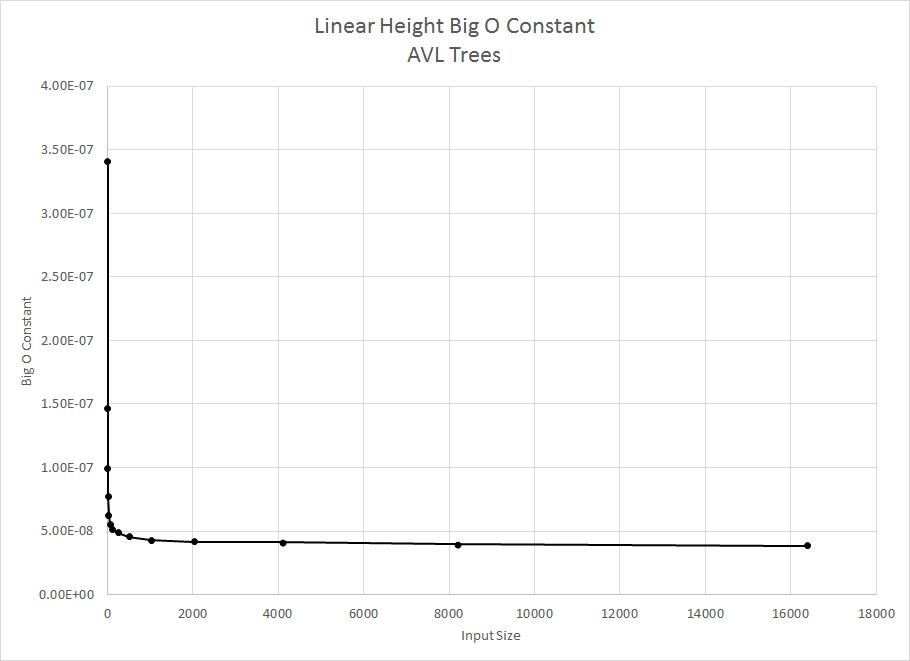
\includegraphics[width=11cm]{report/Linear_Big_O_(AVL)} \caption{Graph of the Big O Constants for Different Input Sizes for a Linear
Order Added AVL Tree}
\label{fig:Linear_Big_O_AVL} 
\end{figure}

\noindent The first set of timing tests that were run on the code were for linearly inserted elements. This means that were the structure of the tree not changed by rebalancing, the tree would have a height that is $O(n)$, where $n$ is the number of nodes in the tree. These tests should result in the worst case for the insertions. This test was first run on the normal binary search tree then it was run on the AVL tree. As was predicted by the theoretical analysis, the time taken by the normal binary search tree was $O(n)$ (because $h$ is $O(n)$). This is seen in Figure~\ref{fig:Linear_Time_Per_Binary} where the time per one insertion goes up basically linearly with respect to the input size. In contrast, the AVL tree runs in $O(\log{n})$ time, as is clearly seen in the logarithmic shape of the graph in Figure~\ref{fig:Linear_Time_Per_AVL}. As further confirmation that the results behaved as was expected, the Big O constants were calculated in both cases. They were calculated by dividing the time per insertion by the expected time for each insertion, which is $n$ for the regular binary search tree and $\log{n}$ for the AVL tree. The graphs of both of these results (Figures~\ref{fig:Linear_Big_O_Binary} and~\ref{fig:Linear_Big_O_AVL}) flatten out for their larger input sizes, suggesting that the flattened value is the Big O constant. The Big O constant for the binary search tree was $1*10^{-8}$ and for the AVL tree was $5*10^{-8}$. The Big O constant is actually larger for the AVL tree than for the binary search tree. This is inconsequential, however, because their Big O functions are not the same. Comparing Big O constants is only meaningful when the functions are the same. In this case, for larger input values (i.e. asymptotically) the binary search tree will be much slower because $O(n)$ is much larger than $O(\log{n})$.\\


\begin{figure}[h]
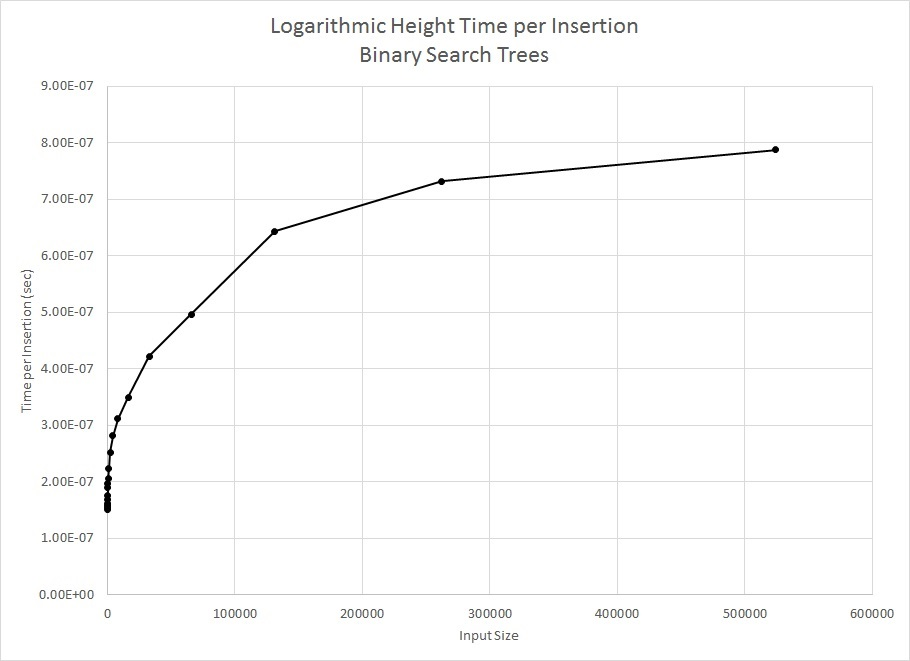
\includegraphics[width=11cm]{report/Logarithmic_Time_Per_(Binary)}
\caption{Graph of the Time Taken per Addition for Different Input Sizes for
a Logarithmic Order Added Binary Search Tree}
\label{fig:Logarithmic_Time_Per_Binary} 
\end{figure}


\begin{figure}[h]
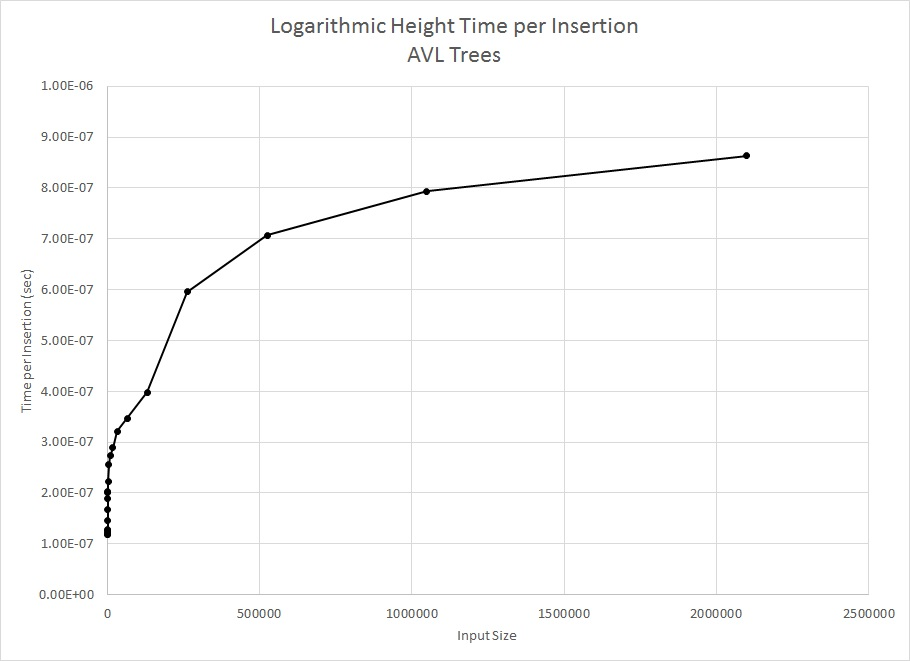
\includegraphics[width=11cm]{report/Logarithmic_Time_Per_(AVL)} \caption{Graph of the Time Taken for Different Input Sizes for a Logarithmic
Order Added AVL Tree}
\label{fig:Logarithmic_Time_Per_AVL} 
\end{figure}


\begin{figure}[h]
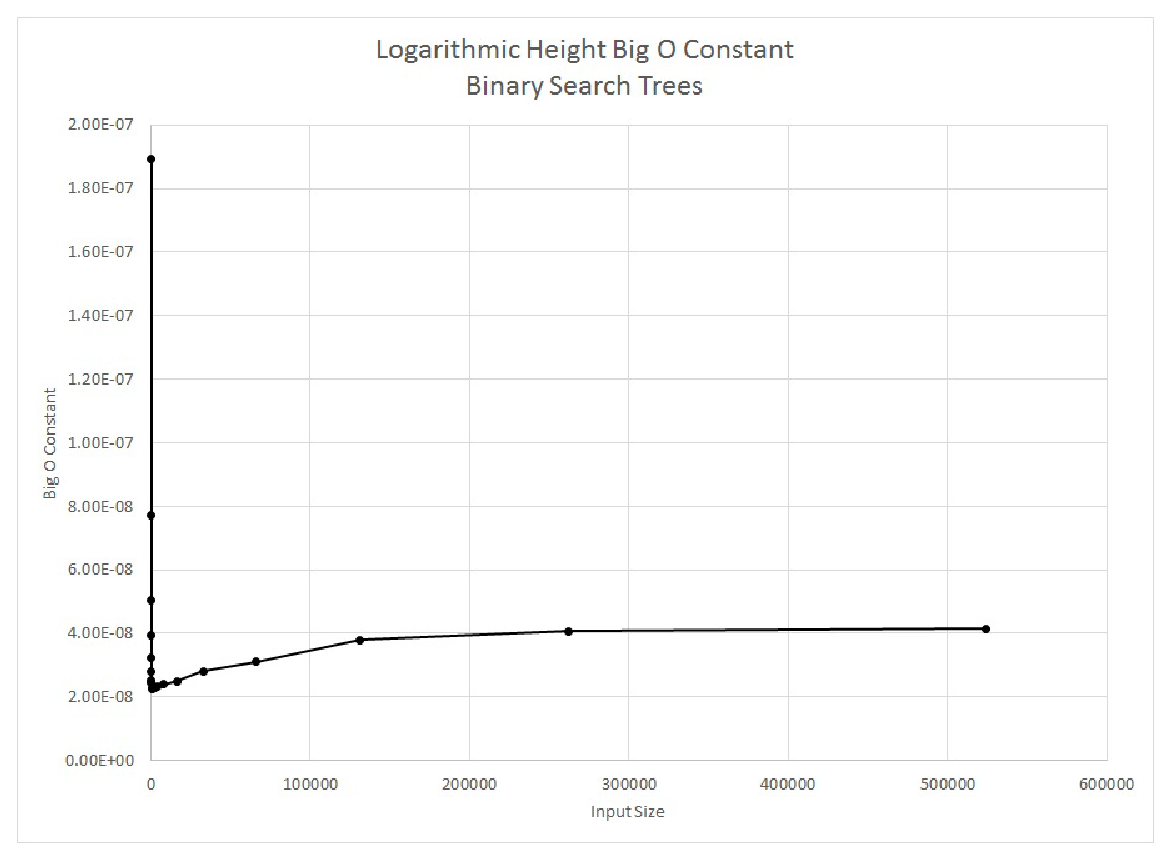
\includegraphics[width=11cm]{report/Logarithmic_Big_O_(Binary)} \caption{Graph of the Big O Constants for Different Input Sizes for a Logarithmic
Order Added Binary Search Tree}
\label{fig:Logarithmic_Big_O_Binary} 
\end{figure}


\begin{figure}[h]
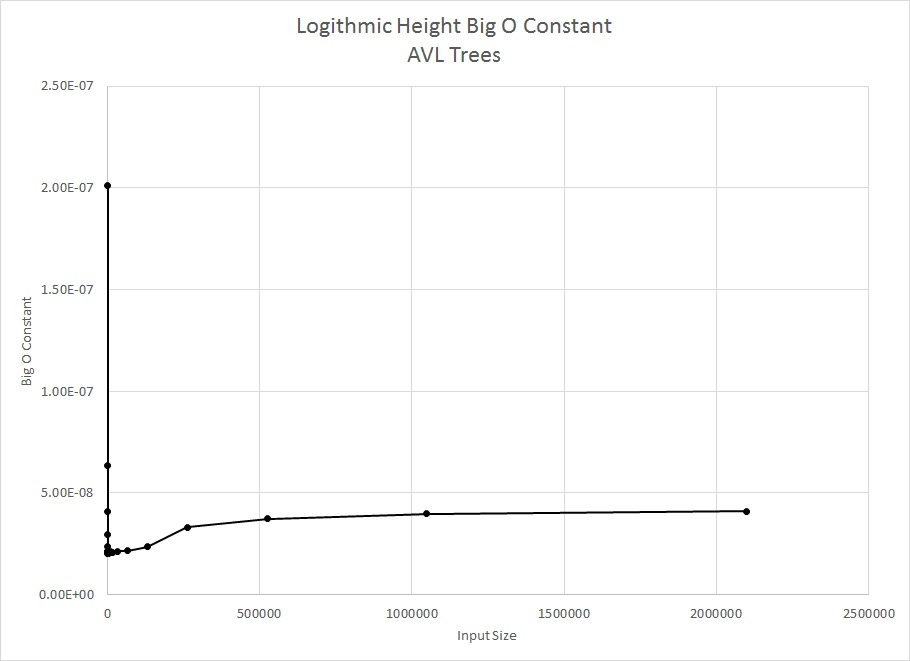
\includegraphics[width=11cm]{report/Logarithmic_Big_O_(AVL)} \caption{Graph of the Big O Constants for Different Input Sizes for a Logarithmic
Order Added AVL Tree}
\label{fig:Logarithmic_Big_O_AVL} 
\end{figure}


\noindent The next set of tests that were run on the code were with logarithmically inserted element. This means that the structure of the tree would be logarithmic if it was not changed by rebalancing. These tests should be the best case for the insertions. Like the last tests, these tests were run on the binary search tree first then on the AVL tree. Again, the results agreed with the theoretical predictions made earlier. The results for the time taken per insertion with respect to input size for the binary search tree were $O(\log{n})$ this time, as is seen in Figure~\ref{fig:Logarithmic_Time_Per_Binary}. This is still $O(h)$; it is just that $h$ is now $O(\log{n})$ instead of $O(n)$ as it was in the last case. Also, as was expected, the results for the AVL tree were $O(\log{n})$ (Figure~\ref{fig:Logarithmic_Time_Per_AVL}). The agreement between the theoretical and actual results was more strongly confirmed when looking at the Big O constants for the insertions in the binary search tree and the AVL tree. The Big O constants were again calculated by dividing the time per insertion by the expected time per insertion. In this case the expected time for insertion for both the binary search tree and the AVL tree were $\log{n}$. In both cases, the results for the Big O constants flattened out for larger input sizes (Figures~\ref{fig:Logarithmic_Big_O_Binary} and~\ref{fig:Logarithmic_Big_O_AVL}), suggesting that the constants are correct, as are the Big O functions. The Big O constant appears to be about $4*10^{-8}$ for the binary search tree and $4*10^{-8}$ for the AVL tree as well. These constants may actually be compared this time because the Big O functions were the same ($O(\log{n})$). In this case they have approximately the same constant. This means that they should take approximately the same amount of time. This is significant because it shows that the overhead for the checks in restructuring are not significant. The actually time taken for restructures cannot be determined because they were not needed for this tree shape, but the checks still occurred and had no discernible impact on the Big O constant. \\


\begin{figure}[h]
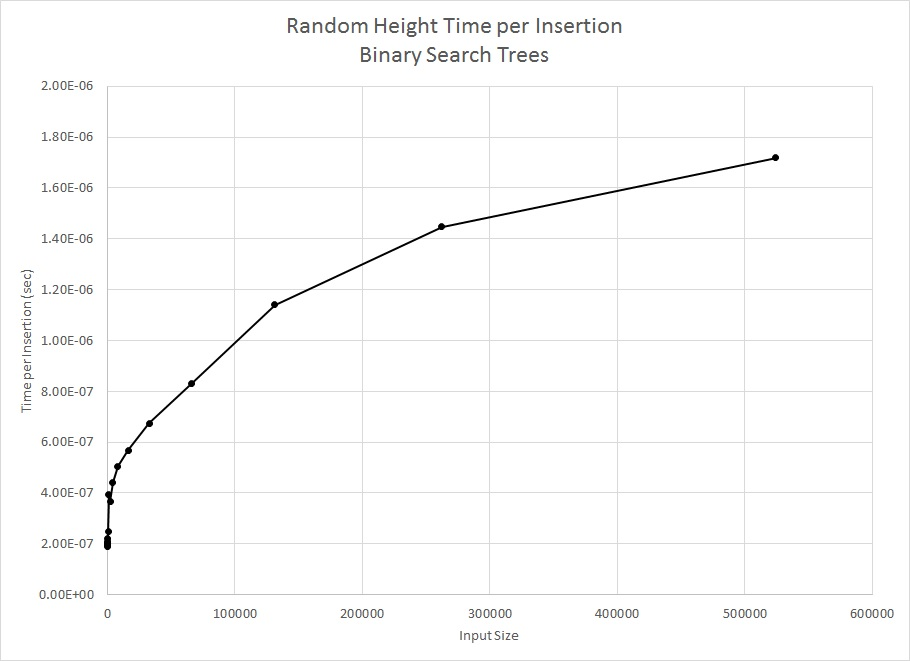
\includegraphics[width=11cm]{report/Random_Time_Per_(Binary)} \caption{Graph of the Time Taken per Addition for Different Input Sizes for
a Random Order Added Binary Search Tree}
\label{fig:Random_Time_Per_Binary} 
\end{figure}


\begin{figure}[h]
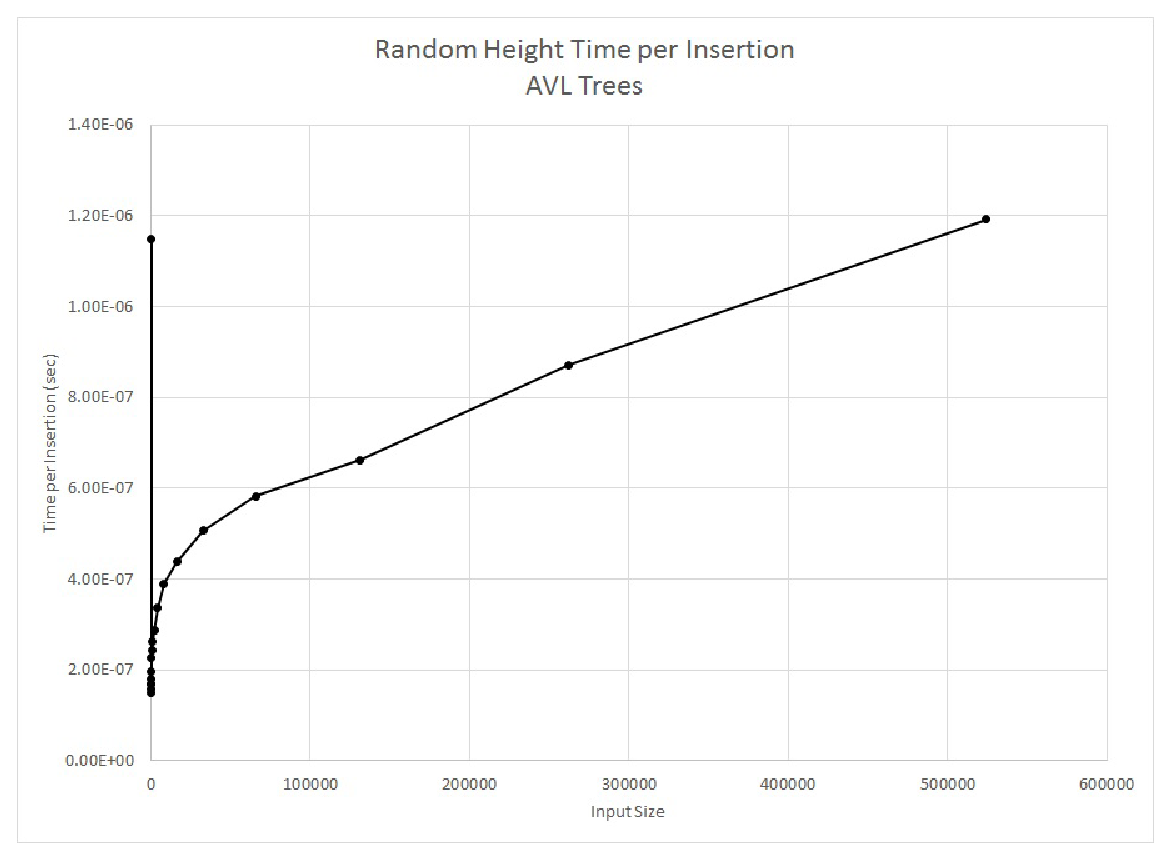
\includegraphics[width=11cm]{report/Random_Time_Per_(AVL)} \caption{Graph of the Time Taken for Different Input Sizes for a Random Order
Added AVL Tree}
\label{fig:Random_Time_Per_AVL} 
\end{figure}


\begin{figure}[h]
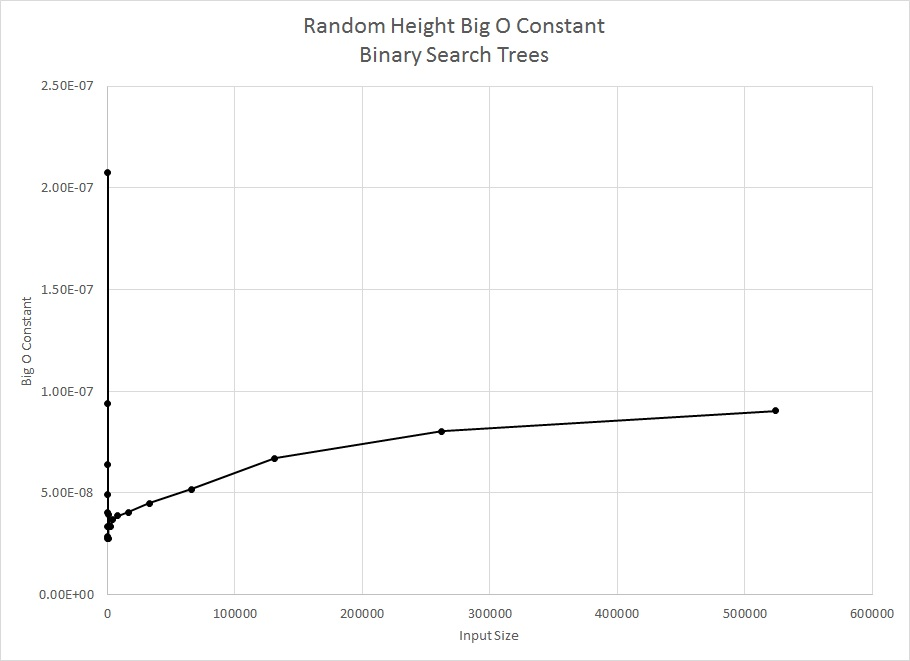
\includegraphics[width=11cm]{report/Random_Big_O_(Binary)} \caption{Graph of the Big O Constants for Different Input Sizes for a Random
Order Added Binary Search Tree}
\label{fig:Random_Big_O_Binary} 
\end{figure}


\begin{figure}[h]
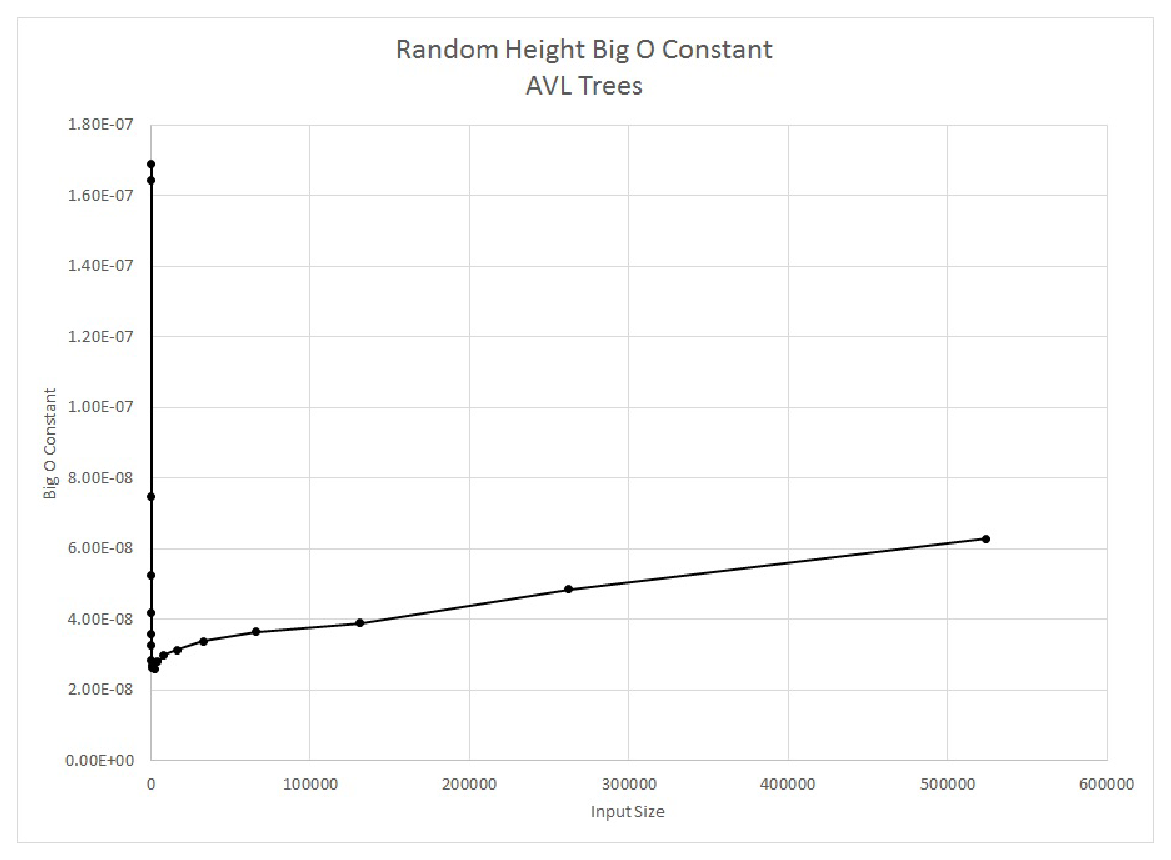
\includegraphics[width=11cm]{report/Random_Big_O_(AVL)} \caption{Graph of the Big O Constants for Different Input Sizes for a Random Order Added AVL Tree}
\label{fig:Random_Big_O_AVL} 
\end{figure}


\noindent The last tests that were run were intended to test the average case for the insertion. This case was the randomly inserted case where elements were put in the tree in no particular order. The shape of this tree before restructuring could be anywhere between logarithmic and linear. The test were run for both the binary search tree and the AVL tree. The results for both types of trees where what was predicted. The results for the time taken per insertion for a binary search tree were $O(\log{n})$ as can be seen in the graph in Figure~\ref{fig:Random_Time_Per_Binary}. Since on average the height of a binary search tree will be $O(\log{n})$, $O(h) = O(\log{n})$, so the results agree with the predictions. The results for the AVL tree (Figure~\ref{fig:Random_Time_Per_AVL}) show that the insertion for the AVL tree with random trees is also $O(\log{n})$. This agrees with the theoretical analysis that operations on the AVL tree are always $O(\log{n})$. The Big O constants were calculated for both the binary search tree and the AVL tree. The function that they were both compared to was $\log{n}$. The graphs of the Big O constants ((Figures~\ref{fig:Random_Big_O_Binary} and~\ref{fig:Random_Big_O_AVL}) basically flattened out, showing that the correct Big O function was chosen. The graphs do not quite flatten out. This is possibly because the randomness of the inputs was not quite normalized by the input size. The Big O constant for the binary search tree was about $9*10^{-8}$ while the constant for the AVL tree was about $6*10^{-8}$. Since both functions are $O(\log{n})$, their Big O constants can be compared. The fact that the constant for the AVL tree is smaller than that of the binary search tree, it can be determined that the AVL tree is better on average. The cost that AVL trees get in restructuring the elements is less than the cost that the binary search tree gets in having taller trees. \\

\noindent When comparing the performance of the insertion for either the binary search tree or the AVL tree, the worst and best cases can be determined. The results show that the worst, best, and average cases are what they were expected to be. For the binary search tree, the linear case was obviously the worst case because it was $O(n)$ while the other two cases were $O(\log{n})$. Looking at the remaining cases, logarithmic is the best case because it has a Big O constant of $4*10^{-8}$ while the random case has a Big O constant of $9*10^{-8}$. The same order holds for the AVL tree. Since its insertions were all $O(\log{n})$, the cases can be ordered solely by Big O constants. Since the linear case has fewer inputs, it is important to measure the Big O constants around the highest input size that the linear case received, 16384. The Big O constants for the linear, logarithmic, and random cases around that point are $5.0*10^{-8}$, $2.5*10^{-8}$, and $4*10^{-8}$, respectively. That means that the best case is the logarithmic case and the worst case is the linear case, as was expected.


\section*{Conclusion}

This assignment achieved a few main goals. First and foremost, it deepened the understanding of the way maps and binary search trees work. It also introduced, in a practical way, how to use AVL trees. It also verified the theoretical discussions that are had in class about the performance of functions of the ADT implementation. The advantages of the AVL tree were concretely seen in the performance difference between the regular binary search tree and an AVL tree. From the timing results measured in this assignment, it can be seen that AVL trees are better than or on par with binary search trees in every situation. Overall, this assignment as a whole gave needed practice in coding as well as reinforced concepts that were learned in class.
\end{document}

